\chapter{Omnicar Platform, ROS Integration and High-Level Software Architecture }

  \section{High-Level Software Architecture: From ROS1 Noetic to ROS2 Jazzy}
  In this thesis, the previous ROS1-based architecture was progressively migrated to ROS2 Jazzy.
  The objective wasn't to update the software stack, but also to obtain a structure that could be tested more easily, extended with new modules, and maintained on the Raspberry Pi 5.

  The transition to ROS2 was particularly relevant for this platform because the high-level software has to coordinate several modules: the serial driver, the odometry node, the localization pipeline, the lidar interface, and the motion-control nodes. In this context, the \textbf{Data Distribution Service} based communication layer of ROS2 provides a more suitable basis for distributed execution and future extensions than the previous centralized \textbf{ROS Master}.

  The hardware upgrade to the \textbf{Raspberry Pi 5} was also an important part of the migration. Compared with the \textbf{Raspberry Pi 3} used in the previous version, the new board offers more computational margin for running several ROS2 nodes at the same time. This is especially useful for odometry computation, localization, lidar data processing, and high-level control tasks, where delays or CPU saturation can directly affect the quality of the robot behaviour.

  \subsection{Migration and Local Implementation}
  From a practical point of view, the migration required rebuilding the software stack around the ROS2 workflow and checking each module separately before running the complete robot. This was necessary because the driver, odometry, localization, and control nodes depend on each other, but failures in one layer can easily mask problems in the others.

  During the migration, I chose to keep the project inside a dedicated ROS2 workspace on the Raspberry Pi instead of mixing the packages with system-level software. This made the development process easier to control, especially when rebuilding packages, changing configuration files, or testing only a subset of the nodes.

  \begin{itemize}
      \item \textbf{Dependency Isolation}: A local workspace allows better control
  of project-specific dependencies and reduces conflicts with system-wide
  libraries and packages.
      \item \textbf{Package organization}: The workspace structure helps organize drivers,
  interfaces, launch files, and configuration files in a clear and maintainable
  way.
      \item \textbf{Reproducibility}: The complete software can be deployed more
  easily on different Raspberry Pi boards while preserving the same internal
  package organization.
      \item \textbf{Future Extensions}: ROS2 makes future extensions easier, such as
  improved localization, additional sensors, and more advanced control features.
  \end{itemize}

  The migration was not limited to a simple syntax update. Some technical points
  required particular attention during the transition:

  \begin{itemize}
      \item the change from the ROS1 \texttt{catkin} build system to the ROS2
  \texttt{ament\_cmake} and \texttt{colcon} workflow;
      \item the adaptation of legacy custom messages and services to the ROS2
  interface package \texttt{sdpo\_drivers\_interfaces};
      \item the conversion of launch files to the ROS2 Python-based launch system;
      \item the verification of topic names, node names, parameter files, and TF
  frame conventions;
      \item the preservation of compatibility with the serial protocol used by the
  ESP32 firmware.
  \end{itemize}

  For this reason, the migration was performed progressively. I first focused on the ROS2 driver, because it represented the mandatory bridge between the Raspberry Pi and the ESP32 firmware. Once this communication layer was stable, the remaining modules could be migrated and tested one at a time.

  \subsection{Workspace Structure}
  The active ROS2 workspace of the project is \texttt{omnicar\_ws}. It follows the
  standard ROS2 and \texttt{colcon} organization, where the compiled artifacts are
  separated from the source code. In particular, the directories \texttt{build/},
  \texttt{install/}, and \texttt{log/} contain the compilation results and runtime
  environment, while the \texttt{src/} directory contains the software packages
  under development.

  Each package keeps the standard ROS2 files, namely \texttt{CMakeLists.txt} and \texttt{package.xml}, which define the build targets, dependencies, and package metadata.

  The separation between header files (\texttt{.h}) and source files
  (\texttt{.cpp}) remains important for code organization and maintainability.
  Header files define the interfaces of the software components, while source
  files implement the internal logic. This structure simplifies development and
  supports incremental compilation.

  The \texttt{config} directories use \texttt{.yaml} files to store parameters
  such as communication settings, odometry constants, and localization
  configuration. This choice makes the system easier to configure and tune without
  modifying the source code.

  The following directory tree shows the simplified structure of the active ROS2
  workspace:

\begin{folderbox}{omnicar\_ws: Simplified Structure}
\begingroup
\scriptsize
\renewcommand{\baselinestretch}{0.85}\selectfont
\dirtree{%
.1 omnicar\_ws/.
.2 bags/ \DTcomment{Recorded ROS2 bag files from controller and robot tests}.
.2 Test/ \DTcomment{Offline analysis workspace for experimental validation}.
.3 test\_code/ \DTcomment{Python scripts and configuration files for bag analysis}.
.3 test\_results/ \DTcomment{Generated plots, metrics and summaries from test runs}.
.2 src/ \DTcomment{ROS2 source workspace containing robot packages and support libraries}.
.3 5dpo\_ratf\_driver-main/ \DTcomment{Main ROS2 robot driver package}.
.4 include/ \DTcomment{Header files for robot and driver classes}.
.4 src/ \DTcomment{ROS2 source files, including driver and tuning nodes}.
.4 launch/ \DTcomment{ROS2 launch files, including bringup}.
.4 sh/ \DTcomment{Support scripts and legacy tuning utilities}.
.3 sdpo\_driver\_omnijoy/ \DTcomment{ROS2 joystick teleoperation node}.
.4 src/ \DTcomment{Joystick command processing logic}.
.4 launch/ \DTcomment{Launch file for Logitech F710 teleoperation}.
.3 sdpo\_drivers\_interfaces/ \DTcomment{ROS2 custom messages and services}.
.4 msg/ \DTcomment{Motor reference and encoder feedback messages}.
.4 srv/ \DTcomment{Custom service definitions}.
.3 sdpo\_ros\_odom/ \DTcomment{ROS2 odometry computation package}.
.4 include/ \DTcomment{Odometry class headers}.
.4 src/ \DTcomment{Odometry implementation}.
.4 config/ \DTcomment{Kinematic and wheel parameters}.
.4 launch/ \DTcomment{Odometry launch files}.
.3 sdpo\_ratf\_ros\_localization/ \DTcomment{ROS2 localization module}.
.4 include/ \DTcomment{Localization and EKF headers}.
.4 src/ \DTcomment{Localization implementation}.
.4 config/ \DTcomment{Localization parameters}.
.4 launch/ \DTcomment{Localization launch file}.
.3 ldlidar\_stl\_ros/ \DTcomment{ROS2 lidar integration package}.
.4 src/ \DTcomment{Lidar publishing and listening nodes}.
.4 config/ \DTcomment{Lidar configuration files}.
.3 5dpo\_serial\_port-main/ \DTcomment{Asynchronous serial communication library}.
.4 include/ \DTcomment{Serial communication headers}.
.4 src/ \DTcomment{Async serial implementation}.
.3 serial\_communication\_channels-main/ \DTcomment{Serial channel protocol library}.
.4 include/ \DTcomment{Protocol headers}.
.4 src/ \DTcomment{Protocol implementation}.
.3 sdpo\_motion\_control/ \DTcomment{High-level ROS2 motion-control package}.
.4 config/ \DTcomment{Controller parameter files and trajectory/path settings}.
.4 src/ \DTcomment{Controller node implementations for go-to-point and path following}.
.4 launch/ \DTcomment{Launch files for controller tests}.
.4 msg/ \DTcomment{Custom debug messages published by the control nodes}.
}
\endgroup
\end{folderbox}



 \subsection{Experimental Validation: ROS2 Integration and Control Chain}
  This phase of the software integration focused on validating the
  communication and control chain of the OmniCar platform in the ROS2 environment.
  These tests were intended to verify the correctness of serial communication with
  the ESP32 controller, the consistency of encoder feedback, joystick commands, odometry, and localization modules inside the migrated ROS2 architecture.

  \subsubsection{Test 1: Encoder Monitoring and Open-Loop Velocity Control}
  The first test was intentionally simple, because before testing odometry or control it was necessary to verify that the Raspberry Pi could receive reliable encoder data from the ESP32.

  \paragraph{Operational Procedure}
  After enabling access to the serial device, the main driver node,
  \texttt{sdpo\_ratf\_driver}, was launched. This node is the central
  communication interface between the ROS2 graph and the ESP32 firmware. In the
  current implementation, it subscribes to the \texttt{motors\_ref} topic and
  publishes encoder and digital state feedback through the topics
  \texttt{motors\_enc}, \texttt{switch\_1\_state}, and \texttt{switch\_2\_state}.
  
  \vspace{0.2cm}
  
  To validate the feedback chain, the \texttt{motors\_enc} topic was monitored
  during runtime while the wheels were rotated manually. This check confirmed the
  correct reception of encoder increments, the absence of packet loss, and the
  correct transmission of angular speed and ticks-per-revolution information from
  the embedded layer to ROS2.

  \vspace{0.2cm}
  
  For actuation validation, a constant reference was sent on the
  \texttt{motors\_ref} topic using the custom message type
  \texttt{sdpo\_drivers\_interfaces/msg/MotRefArray}. In this way, it was possible
  to verify the complete command path from ROS2 to the ESP32 firmware.

  The test confirmed that the node \texttt{sdpo\_ratf\_driver} acts as the central
  bridge of the low-level architecture. It guarantees bidirectional data exchange
  with the embedded controller while providing a stable interface for the higher-
  level ROS2 nodes.

\begin{figure}[H]
    \centering
    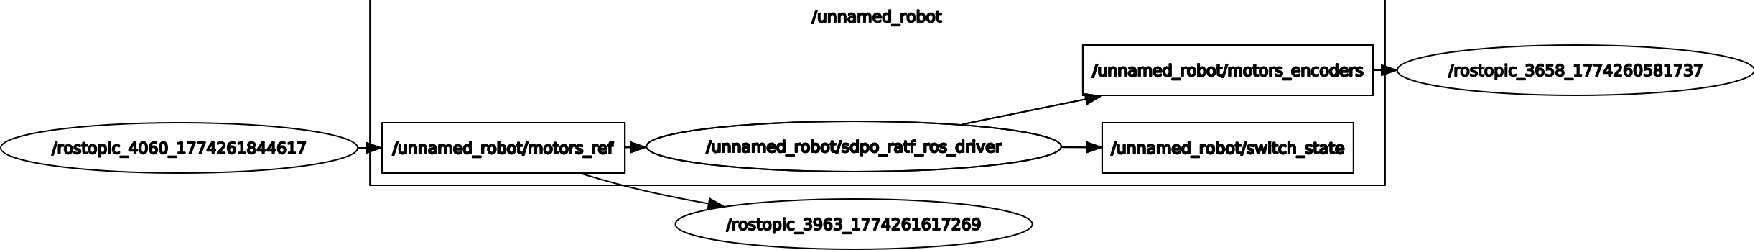
\includegraphics[width=1.1\textwidth]{IMG/ROS/PDF_rosgraph_test_enc_vel_ref.pdf}
    \caption{rqt\_graph showing the active nodes and topics during the encoder test, including reference velocity and measured encoder feedback.}
    \label{fig:rqt_graph_test_Encoder}
\end{figure}

\begin{vscode}{Commands to use for Test 1}
CMD1  
  ros2 launch sdpo_ratf_driver sdpo_ratf_driver.launch.py

CMD2
  ros2 topic echo /unnamed_robot/motors_enc

CMD3
  ros2 topic pub -r 20 /unnamed_robot/motors_ref sdpo_drivers_interfaces/msg/MotRefArray "{ang_speed_ref: [{ref: 5.0}, {ref: 5.0}, {ref: 5.0}, {ref:5.0}]}"
  ros2 topic pub -r 20 /unnamed_robot/motors_ref sdpo_drivers_interfaces/msg/MotRefArray "{ang_speed_ref: [{ref: 0.0}, {ref: 0.0}, {ref: 0.0}, {ref:0.0}]}"
\end{vscode}

  \subsubsection{Test 2: Manual Control using a Joystick Controller}
  The second validation phase concerned the integration of a joystick controller
  in the ROS2 environment, with the aim of verifying manual control of the
  platform and the correct interaction between high-level user commands and low-
  level motor actuation.

  The teleoperation chain is organized into three stages:
  \begin{itemize}
      \item \textbf{Joystick Acquisition}: The node \texttt{joy\_linux\_node},
  launched through the package \texttt{joy\_linux}, acquires the state of the
  Logitech F710 controller and publishes it on the topic \texttt{joy} as
  \texttt{sensor\_msgs/msg/Joy}.
      \item \textbf{User Command Interpretation}: The node
  \texttt{sdpo\_driver\_omnijoy} subscribes to \texttt{joy} and converts the
  joystick inputs into a velocity command of type \texttt{geometry\_msgs/msg/
  Twist}, published on the topic \texttt{cmd\_vel}. This node applies deadman
  logic and scaling factors for linear and angular motion.
      \item \textbf{Conversion into Wheel References}: The node
  \texttt{sdpo\_ros\_odom\_cmd\_vel} subscribes to \texttt{cmd\_vel}, applies the
  inverse kinematics of the four-wheel omnidirectional platform, and publishes the
  resulting wheel references on \texttt{motors\_ref}. In addition, it publishes
  the scaled robot-level reference on \texttt{cmd\_vel\_ref}.
  \end{itemize}

  At this point, the node \texttt{sdpo\_ratf\_driver} receives the
  \texttt{motors\_ref} message and transmits the corresponding angular speed
  references to the ESP32 firmware through the serial communication protocol.

  This result is important, because it shows that the migrated ROS2 control chain is modular and separated into functional layers. The joystick node manages the user input, the kinematic conversion node computes the wheel references, and the main driver handles
  communication with the embedded controller. This separation improves clarity,
  maintainability, and testability of the overall system.

  \begin{figure}[H]
    \centering
    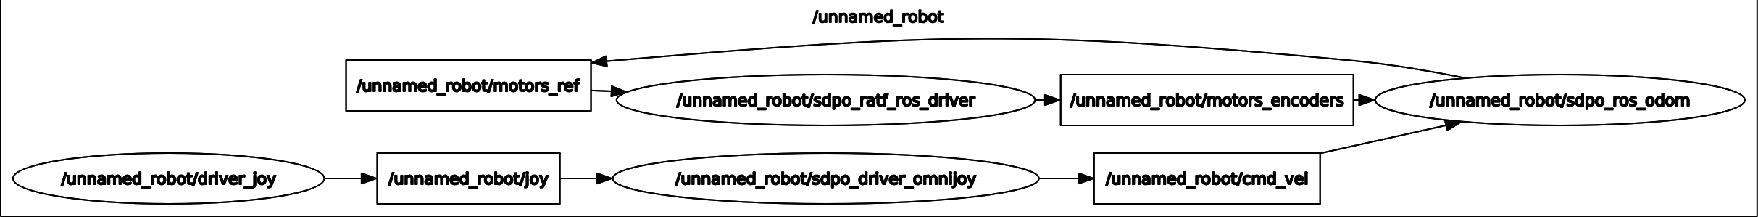
\includegraphics[width=1.1\textwidth]{IMG/ROS/PDF_rosgraph_test_joystick.pdf}
    \caption{rqt\_graph showing the active nodes and topics during the joystick test}
    \label{fig:rqt_graph_test_joy}
\end{figure}

\begin{vscode}{Commands to use for Test 2}
CMD 1
ros2 launch sdpo_ratf_driver omnicar_joy_control.launch.py

CMD 2
ros2 topic echo /unnamed_robot/odom
\end{vscode}

\vspace{0.4cm}

  \subsubsection{Test 3: Localization and Lidar Integration}
  After validating the joystick teleoperation chain, the next step was to verify that the odometry node produced a coherent estimate of the robot motion. The robot was moved manually or through joystick commands while the estimated pose and TF frames were observed in RViz. The comparison with the real motion showed that the direction of motion and frame alignment were consistent, although small discrepancies appeared due to wheel slip, odometric drift, and modelling errors.

  \vspace{0.2cm}
  
  The localization function is managed by the node
  \texttt{sdpo\_ratf\_ros\_localization}, which subscribes to \texttt{odom} and,
  when enabled, also to \texttt{laser\_scan\_point\_cloud}. It publishes the
  estimated robot pose on the topic \texttt{pose}, the detected beacons on
  \texttt{beacons}, and the reference map beacons as \texttt{map\_beacons}.
  Moreover, it broadcasts the TF transform between the frames \texttt{map} and
  \texttt{odom}.

\vspace{0.2cm}

  This architecture allows localization to refine the odometric estimate by
  combining wheel-based motion prediction with external observations derived from
  the lidar subsystem.
  The localization process can be observed in Fig.~\ref{fig:odom_comparison}, where the RViz visualization shows the lidar scan in red and the detected beacons in white, providing a direct representation of the perception layer used for pose estimation.

\vspace{0.2cm}

  The TF tree adopted in this configuration follows the standard chain \newline 
  \texttt{map} $\rightarrow$ \texttt{odom} $\rightarrow$ \texttt{base\_footprint} $\rightarrow$ \texttt{laser}.
  
   \newline  
   
  In this structure, the \texttt{map} frame represents the global reference, \texttt{odom} provides a continuous but drifting local estimate, \texttt{base\_footprint} defines the robot base frame, and \texttt{laser} corresponds to the lidar sensor frame. This hierarchical organization ensures consistency between localization, odometry, and sensor measurements.

\vspace{0.2cm}

  The lidar integration is provided by the package \texttt{ldlidar\_stl\_ros},
  which publishes scan data for the perception layer. In the current migration
  process, the lidar is an important component because it supports the
  localization pipeline and extends the ROS2 stack beyond basic low-level control.

  The comparison between the real experiment and the RViz visualization shows that the odometry provides a consistent estimate of the robot motion. The trajectory and frame alignment are coherent, while small differences are due to odometric drift, wheel slip, and modeling errors.
  For the following Test, the same laucher used in the previous test is valid.

 \begin{figure}[H]
    \centering

    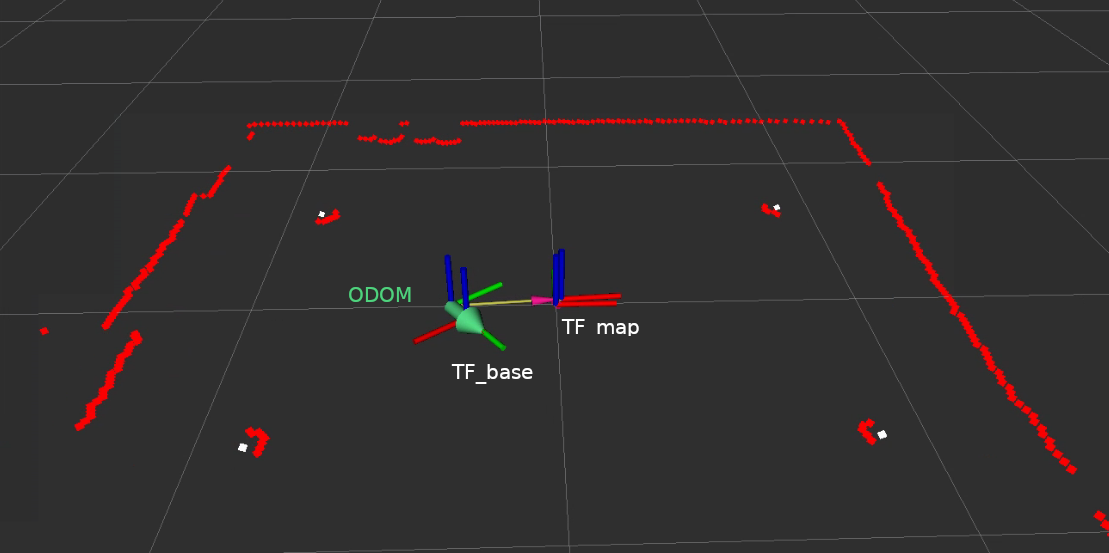
\includegraphics[width=0.90\linewidth]{IMG/ROS/rviz2_odom_edit.png}
    \caption*{RViz odometry and TF visualization}

    \vspace{0.4cm}

    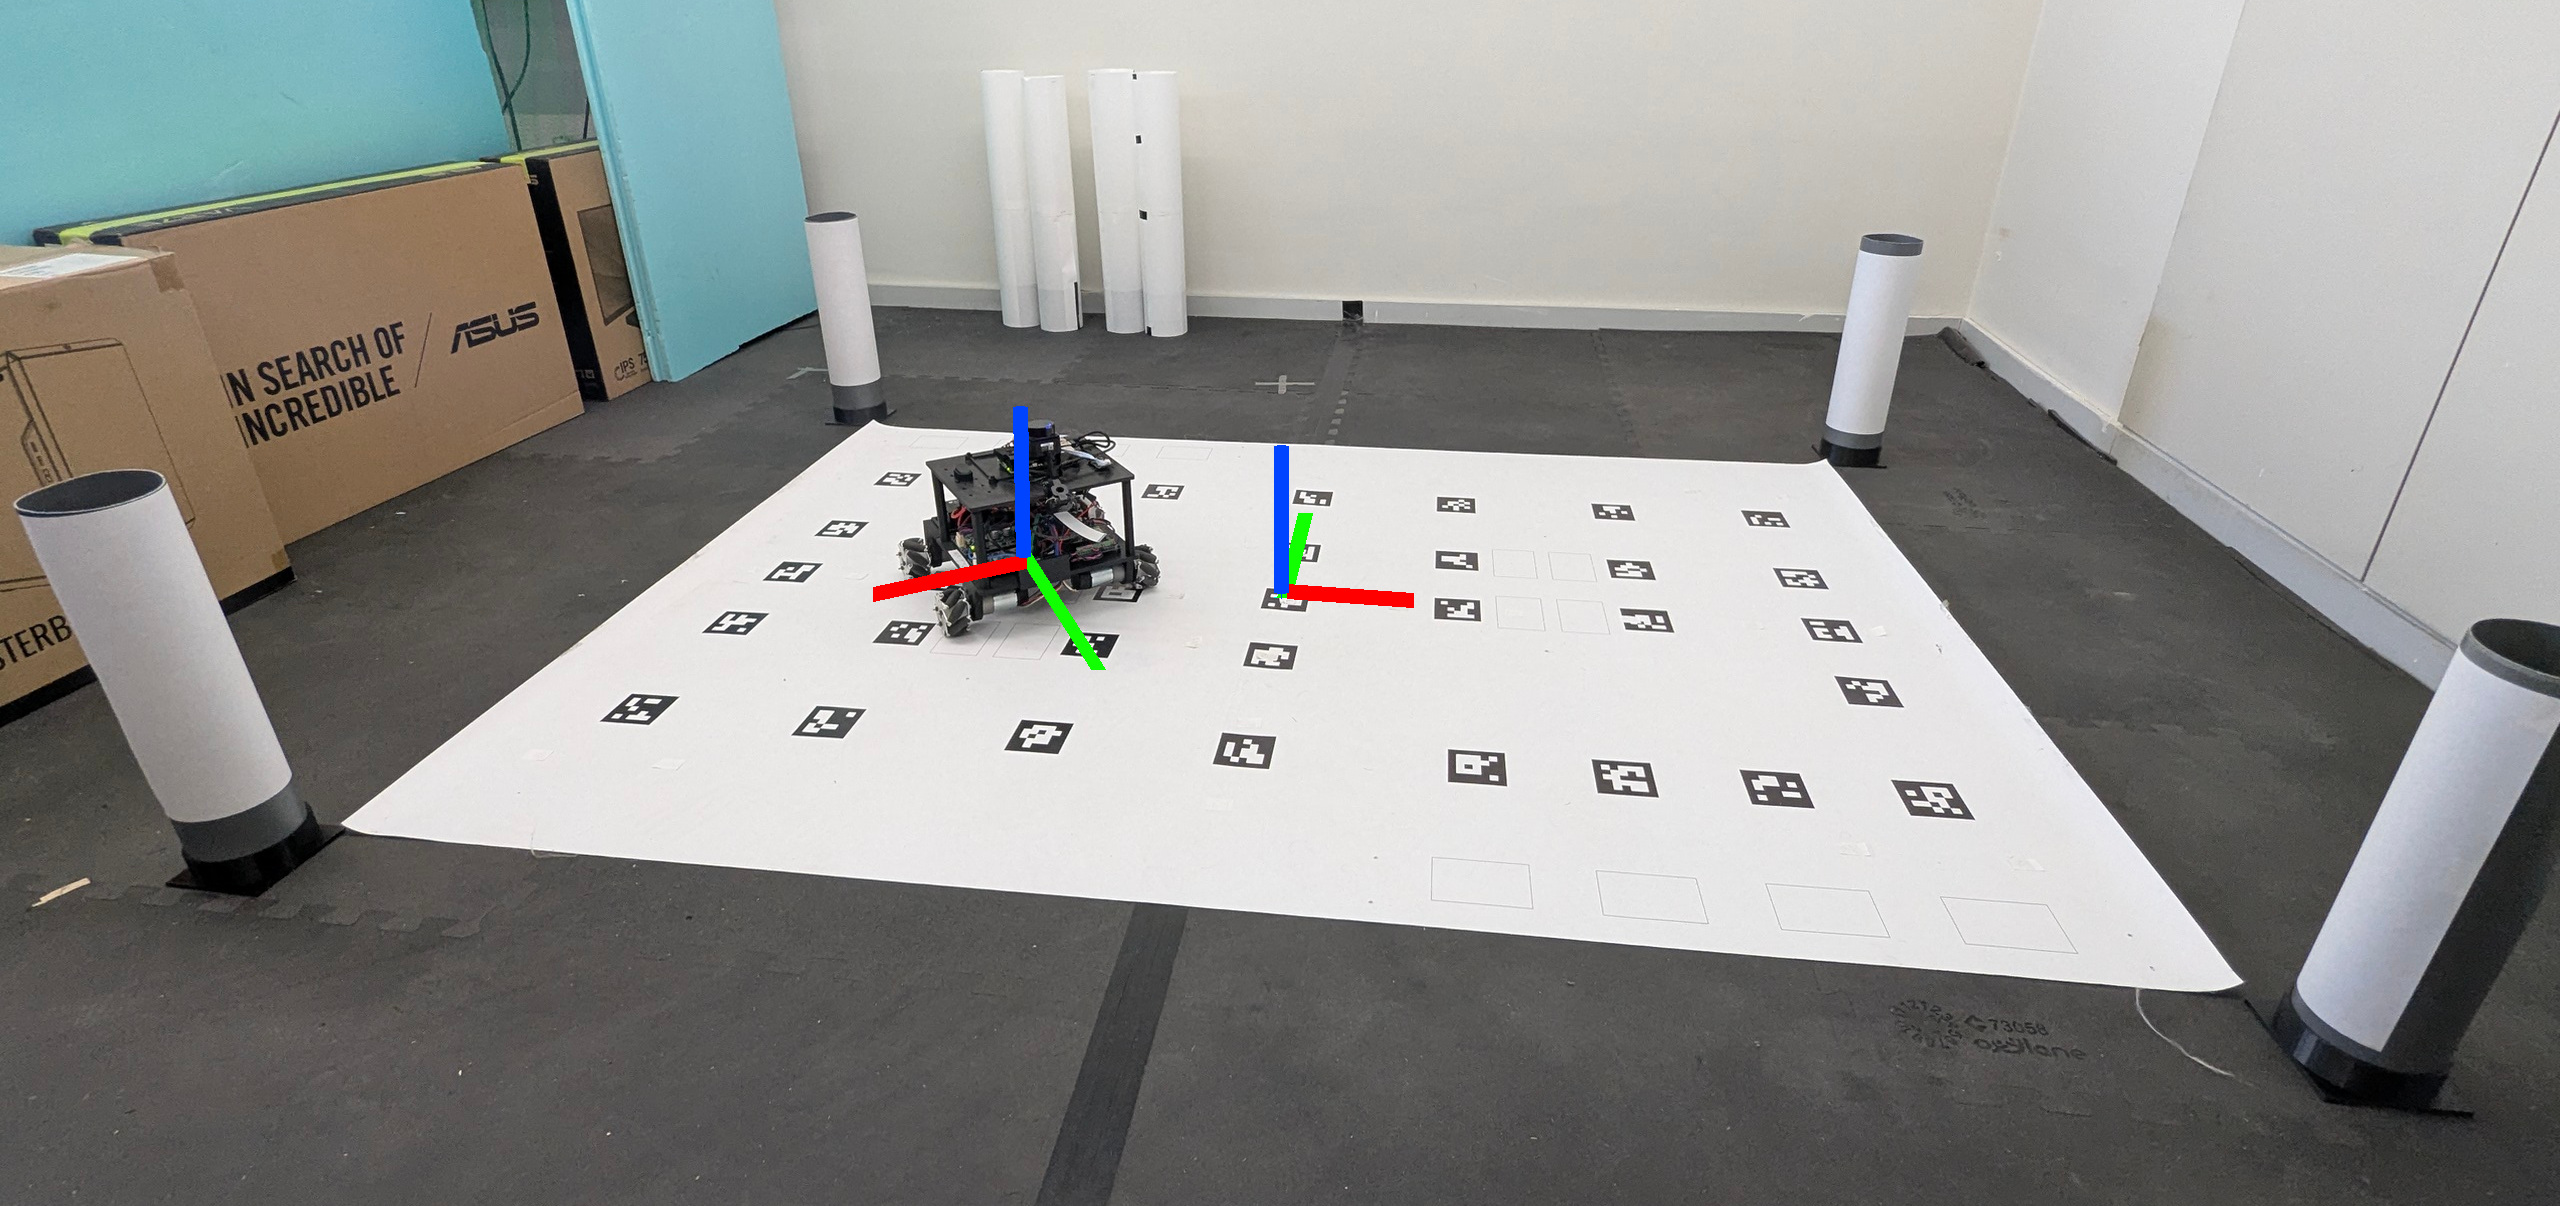
\includegraphics[width=0.90\linewidth]{IMG/ROS/odom_real_edit.jpg}
    \caption*{Real experimental setup}

    \caption{Comparison between the real robot experiment and the corresponding odometry visualization in RViz.}
    \label{fig:odom_comparison}
\end{figure}


\newpage
\subsubsection{Test 4: Waypoint Tracking Validation with the
  \texttt{go\_to\_point} Controller}

  This test represented the first closed-loop high-level motion-control experiment performed within the migrated ROS2 architecture. In this phase, the package \texttt{sdpo\_motion\_control} was used to command the robot toward a
  sequence of planar target poses, with the objective of evaluating the behaviour of the \texttt{go\_to\_point} controller, the consistency of the odometric feedback, and the overall quality of the integrated control chain.

\vspace{0.4cm}

  This test was carried out after correcting an inconsistency in the
  \texttt{map}--\texttt{odom} transformation inside the localization chain. In
  the previous implementation, the rotation between \texttt{map} and \texttt{odom}
  was computed correctly, but the translation term was combined with the robot EKF
  yaw instead of the relative \texttt{map}--\texttt{odom} rotation. This produced a
  frame inconsistency. After this correction, the waypoint experiments became coherent and repeatable.

  \paragraph{Test configuration}
  For controller tuning and validation, six reference poses were assigned in
  sequence. The same six target positions are the ones shown in the plots of
  target trajectory, current robot trajectory, and tracking errors:
  
\begin{figure}[H]
    \centering
    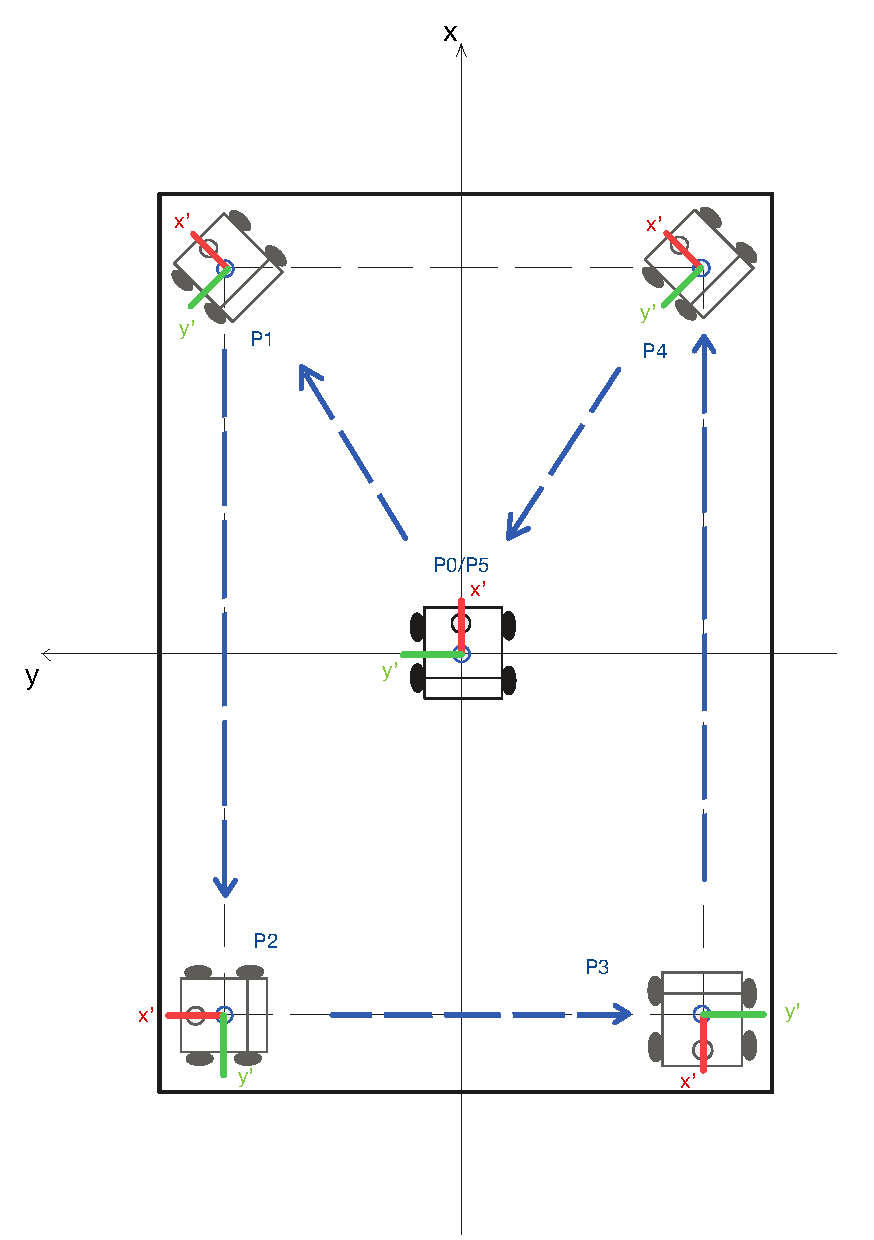
\includegraphics[width=0.52\textwidth]{IMG/ROS/GoToPoint_test_Draw.pdf}
    \caption{diagram of the test executed}
    \label{fig:GoToPoint_test}
\end{figure}

\begin{itemize}
  \item \texttt{(P0) \{x: 0.0, y: 0.0, z: 0.0\}}
  \item \texttt{(P1) \{x: 0.6, y: 0.45, z: 0.78\}}
  \item \texttt{(P2) \{x: -0.6, y: 0.45, z: 1.56\}}
  \item \texttt{(P3) \{x: -0.6, y: -0.45, z: 3.14\}}
  \item \texttt{(P4) \{x: 0.6, y: -0.45, z: 0.78\}}
  \item \texttt{(P5) \{x: 0.0, y: 0.0, z: 0.0\}}
\end{itemize}

    The sequence was chosen to force the robot to move in different directions of the workspace, including diagonal displacements where odometric errors and wheel slip are more visible, ending with a return to the origin.

  \paragraph{Observed behaviour}
  The experiments showed that the \texttt{go\_to\_point} controller is able to
  drive the robot through the assigned sequence and to reach all the commanded
  poses with stable behaviour. Motions along the main axes were generally more
  accurate.

\begin{figure}[H]
    \centering
    \includegraphics[width=1.0\textwidth]{IMG/ROS/TEST4_position.png}
    \caption{plot control position results}
    \label{fig:TEST4_position}
\end{figure}

\begin{figure}[H]
    \centering
    \includegraphics[width=1.0\textwidth]{IMG/ROS/TEST4_position_error.png}
    \caption{plot position errors}
    \label{fig:TEST4_position_error}
\end{figure}

  The comparison between the commanded target pose and the estimated current pose,
  together with the plots of the tracking error, highlighted that the control loop
  remained stable during all tests, but also confirmed the presence of a
  residual positioning error. Over the waypoint sequence, the largest observed deviation was on the order of \(2 \ \mathrm{cm}\) on each
  axis. This discrepancy was not mainly associated with instability of the
  controller itself, but rather with the accumulated estimation error of the
  pose used by the controller.

  The results were particularly useful because they helped separate the effect
  of
  control tuning from the effect of state estimation. In fact, the tests
  confirmed
  that the basic control chain
  \texttt{goal} $\rightarrow$ \texttt{controller} $\rightarrow$
  \texttt{cmd\_vel}
  $\rightarrow$ \texttt{motors\_ref} $\rightarrow$ robot is functionally
  correct,
  while the main limitation at this stage is the residual drift and bias of the
  pose estimate over longer or diagonal displacements.

  \paragraph{Discussion of the results}
  From a control point of view, these experiments represent the first successful
  validation of waypoint regulation in the migrated ROS2 architecture. The robot
  was able to execute repeated planar repositioning tasks using the new
  \texttt{sdpo\_motion\_control} package, and the obtained behaviour is already
  sufficient to consider the controller as a valid baseline for further tuning
  and for future trajectory-tracking developments.

  At the same time, the tests showed that improved precision will require not
  only controller tuning, but also a more accurate calibration of the localization
  and odometry chain, especially for diagonal motions and global return-to-origin
  tasks. For this reason, Test~4 was an important milestone: it validated the
  complete waypoint control loop in ROS2 and clearly identified the remaining
  gap between acceptable closed-loop operation and higher-accuracy autonomous
  navigation.

  \subsection{Final Considerations on the Integrated ROS2 Chain}
From a control perspective, the \texttt{go\_to\_point} validation was carried out within a cascaded control architecture, where the inner loop was already introduced in the previous chapters.

At the embedded level, the ESP32 firmware implements the low-level wheel-velocity regulation loop, including the motor control logic discussed in Chapter~\ref{chap:firmware}. This inner loop tracks wheel-speed references and provides the actuation layer required by the ROS2 motion stack. As a result, the high-level controller running on the Raspberry Pi can be designed at the robot-motion level, in terms of planar pose regulation.

\begin{figure}[H]
    \centering
    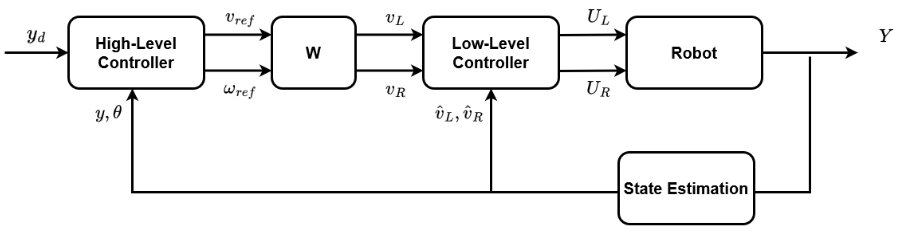
\includegraphics[width=1.0\textwidth]{IMG/controller/controller_general_architecture.png}
    \caption{Controller Architecture}
    \label{fig:Control_Architecture}
\end{figure}

Motion-control architecture adopted for OMNICAR as a two-layer cascade, consistent with the firmware and ROS2 integration described in the previous chapters.

\begin{itemize}
\item \textbf{High-level controller}: receives the estimated robot pose \((x,y,\theta)\) from the state-estimation pipeline and computes robot-level reference velocities for motion tasks (initially waypoint regulation, later path-following scenarios). These references are then mapped to wheel-level commands through the kinematic transformation block \(W\).

\item \textbf{Low-level controller}: implemented on the ESP32, receives wheel-velocity references and applies closed-loop motor control to track them through PWM/DIR actuation, using encoder feedback for regulation.
\end{itemize}

This architecture, shown in Fig.~\ref{fig:Control Architecture}, provides a clear separation of responsibilities: high-level motion generation in ROS2 and fast embedded actuation at firmware level. In the present chapter, the high-level scenario is limited to a \texttt{go\_to\_point} task with a P-only outer loop.

In the ROS2 experiments presented in Test~4, the high-level outer loop was intentionally kept simple and implemented as a \textbf{P-only controller} on the planar coordinates \((x,y,\psi)\). Three proportional actions were used to generate the commanded robot velocities from position and heading errors, while integral and derivative terms were disabled in this phase.

The tuning was performed progressively by starting from moderate proportional gains (around \(K_p \approx 0.8\), then adjusted per axis) and increasing them until a satisfactory compromise between responsiveness and oscillation margin was obtained. This approach was chosen to obtain a robust baseline controller and to isolate the effect of the localization and odometry chain on the final positioning performance.

Experimental results confirmed that this P-only outer loop is sufficient to achieve stable waypoint reaching and repeatable closed-loop behavior for the considered trajectories. Residual errors, especially during diagonal motions and return-to-origin phases, were mainly associated with state-estimation drift and model mismatch rather than with instability of the proportional control law itself.

This test should therefore be interpreted as the first high-level control scenario in the migrated ROS2 architecture: a deliberately simple and transparent baseline. In the next chapter, more advanced high-level control scenarios will be analyzed.


  

